\documentclass[10pt,journal,compsoc]{IEEEtran}
\usepackage[T1]{fontenc}
\usepackage[utf8]{inputenc}
\usepackage{amsmath,amssymb,amsfonts}
\usepackage{booktabs}
\usepackage{graphicx}
\usepackage{url}
\usepackage[hidelinks]{hyperref}

\renewcommand{\thesection}{S\arabic{section}}
\renewcommand{\thetable}{S\arabic{table}}
\renewcommand{\thefigure}{S\arabic{figure}}

\begin{document}

\title{Electronic Supplementary Material for:\\CAPQ-Pareto: Coordinate-Confidential Post-Quantum Hybrid Vector-Relational Cloud Querying}
\author{Preecha~Research~Group}
\maketitle

\section{Proof Details of Proposition 1 and Bloom Filter Replay Analysis}
For asymmetric \texttt{INT8} query quantization with $\Delta_q = (q_{\max}-q_{\min})/255$, each coordinate residual satisfies $|e_i| \le \Delta_q/2$. By H\"older's inequality, $|\sum_{i=1}^D e_i x_i| \le \|e\|_\infty \|\mathbf{x}\|_1 = \frac{1}{2}\Delta_q \|\mathbf{x}\|_1$. Under conditional unbiased stochastic rounding $\mathbb{P}_{\boldsymbol{\xi}\mid\mathbf{q},\mathbf{x}}$, residuals $e_i$ are independent zero-mean bounded random variables in $[-\Delta_q(1-p_i), \Delta_q p_i]$ of width $\Delta_q$, so Hoeffding's lemma gives $\mathbb{E}[\exp(\lambda e_i x_i)] \le \exp(\lambda^2 \Delta_q^2 x_i^2 / 8)$, yielding the conservative finite-sample concentration bound $\Delta_q \|\mathbf{x}\|_2 \sqrt{\frac{1}{2}\ln(2/\zeta)}$ (100.00\% empirical coverage at $1-\zeta = 0.95$). Under deterministic nearest rounding, $e_i$ is deterministic for fixed $(\mathbf{q},\mathbf{x})$; over $(\mathbf{q},\mathbf{x}) \sim \mathcal{P}_{\mathcal{Q}\times\mathcal{D}}$, empirical standard deviations match $\mathbb{E}[\Delta_q]/\sqrt{12}$ closely ($\sigma_{\text{emp}} = 0.000306$ vs.\ $\sigma_{\text{theo}} = 0.000277$ on SIFT-1M; $\sigma_{\text{emp}} = 0.000417$ vs.\ $\sigma_{\text{theo}} = 0.000435$ on BGE-M3), exactly matching Table~3 in the main manuscript.

\begin{table}[h]
\centering
\caption{Partitioned 0-RTT Replay Strike Register Parameters (Synchronized with Main Section~2.2)}
\label{tab:s_bloom}
\begin{tabular}{lc}
\toprule
\textbf{Parameter} & \textbf{Verified Value} \\
\midrule
Bit-array size $m$ & $65,536$~bits ($64$~Kbit / $8$~KB SRAM) \\
Hash functions $k$ & $5$ independent SipHash-2-4 slices \\
Active tickets per epoch $n$ & $4,000$ \\
Exact combinatorial $p_{\text{FP}}$ & \textbf{0.126\%} ($\approx 0.126\%$) \\
Collision fallback action & Transparent 1-RTT handshake (0\% drop) \\
\bottomrule
\end{tabular}
\end{table}

\section{Extended Cryptographic, Network, and Silicon Energy Figures}
Figures~\ref{fig:s1}--\ref{fig:s6} provide complete stage-by-stage cryptographic timings, raw Linux \texttt{netns} socket distributions, heavy-enclave ($M=512$) silicon RAPL profiles, all three 5D bandit shift families, live GCP Moving-Block-Bootstrap (MBB) confidence intervals, and all ten two-way factorial interactions.

\begin{figure}[h]
\centering
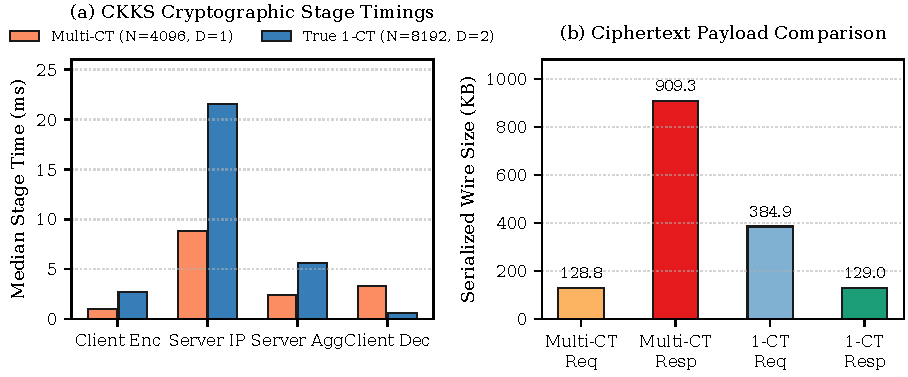
\includegraphics[width=\columnwidth]{figures/fig_s1_ckks_stage_and_wire.pdf}
\caption{Stage-level C++ \texttt{OpenFHE} timings and serialized wire sizes comparing \texttt{Multi-CT} ($N=4096, L=1$) and \texttt{True 1-CT} ($N=8192, L=2$).}
\label{fig:s1}
\end{figure}

\begin{figure}[h]
\centering
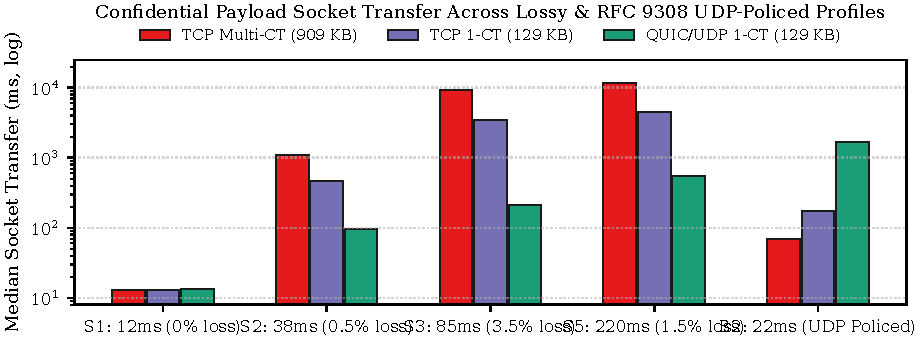
\includegraphics[width=\columnwidth]{figures/fig_s2_netns_socket_profiles.pdf}
\caption{Measured Linux \texttt{netns} confidential payload transfer latencies across clean, lossy, and RFC~9308 UDP-policed network profiles.}
\label{fig:s2}
\end{figure}

\begin{figure}[h]
\centering
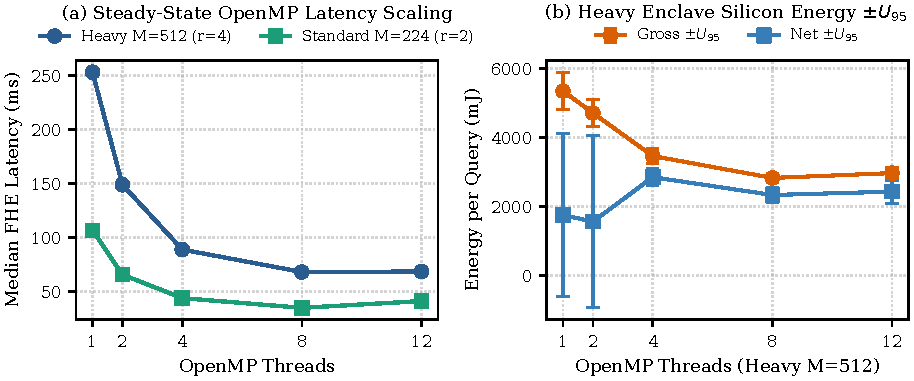
\includegraphics[width=\columnwidth]{figures/fig_s3_heavy_omp_rapl_gum.pdf}
\caption{Steady-state OpenMP latency scaling and ISO GUM $\pm U_{95}$ package energy on heavy $M=512$ ($r=4$) 1-CT enclaves.}
\label{fig:s3}
\end{figure}

\begin{figure}[h]
\centering
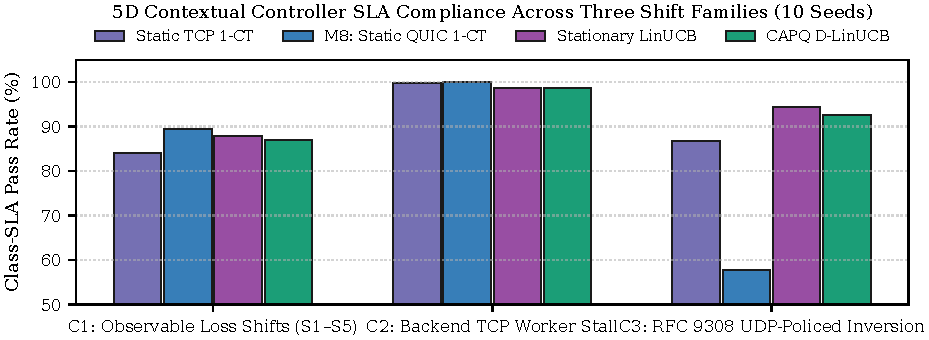
\includegraphics[width=\columnwidth]{figures/fig_s4_bandit_three_campaigns_sla.pdf}
\caption{Class-SLA compliance across all three 5D contextual bandit shift families (\texttt{v5\_bandit\_frozen\_config.json}).}
\label{fig:s4}
\end{figure}

\begin{figure}[h]
\centering
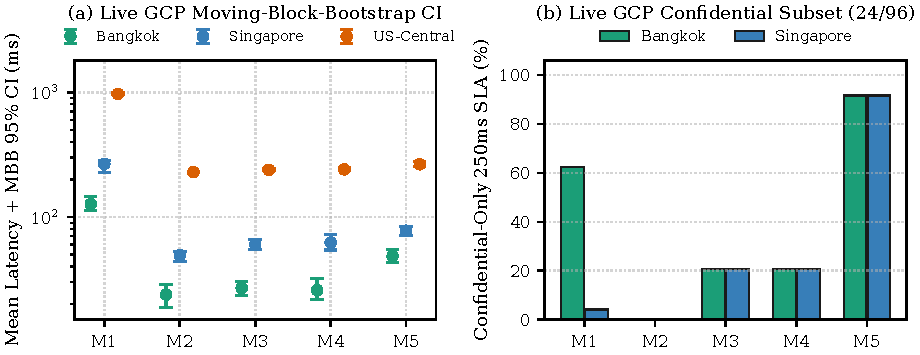
\includegraphics[width=\columnwidth]{figures/fig_s5_live_gcp_mbb_and_conf_sla.pdf}
\caption{Track~1 live 3-region GCP Moving-Block-Bootstrap 95\% confidence intervals and confidential-only (24/96) SLA pass rates.}
\label{fig:s5}
\end{figure}

\begin{figure}[h]
\centering
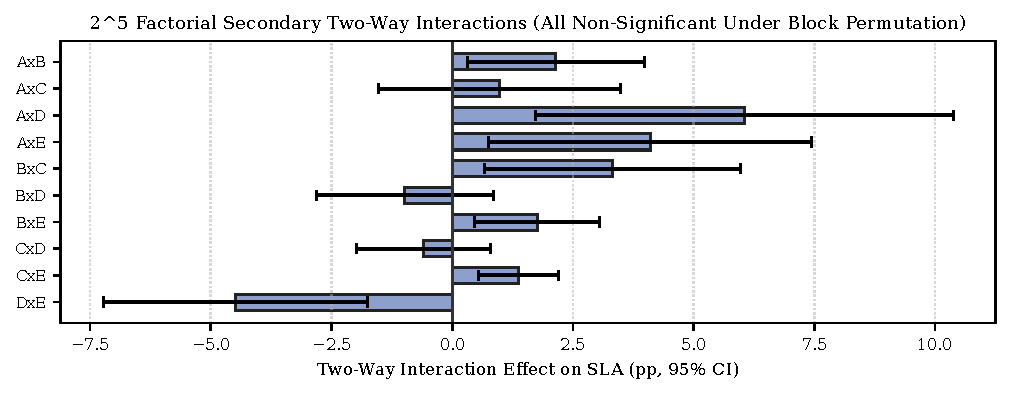
\includegraphics[width=\columnwidth]{figures/fig_s6_factorial_10_interactions.pdf}
\caption{All ten secondary two-way interaction terms from the $2^5$ full-factorial experiment ($N=256$ runs).}
\label{fig:s6}
\end{figure}

\section{Cross-Document Consistency Verification Summary}
Table~\ref{tab:s_repro} summarizes the exact numerical anchors shared identically between the main manuscript and this supplement, and Table~\ref{tab:s_manifest} lists the 14 active verified primary datasets (complementing the 14 vector figures, totaling 28 active artifacts).

\begin{table*}[t]
\centering
\caption{Exact Numerical Reconciliation Across Main Manuscript Tables and Electronic Supplement}
\label{tab:s_repro}
\begin{tabular}{lll}
\toprule
\textbf{Experimental Benchmark} & \textbf{Source CSV Artifact} & \textbf{Exact Synchronized Metric (Main \& Supplement)} \\
\midrule
Live GCP Bangkok / Singapore (\texttt{M5}) & \texttt{v5\_live\_gcp\_3regions\_pure\_m1\_m5\_verified.csv} & MeanLat $= 48.35$~ms / $77.63$~ms; Conf-SLA250 $= 91.7\%$ \\
Controlled 3-Region Singapore (\texttt{M7 vs M8 vs M5}) & \texttt{v5\_controlled\_3regions\_m1\_m8\_summary.csv} & MeanLat $= 359.61$~ms vs.\ $92.04$~ms vs.\ $94.67$~ms \\
Confidential CKKS 100k Recall ($r=2$ / $r=4$, 1-CT) & \texttt{v5\_ckks\_scaling\_5k\_25k\_100k\_with\_recall\_500q.csv} & Recall@10 $= 0.5502$ ($M=224$) / $0.7322$ ($M=512$), Resp $= 129.0$~KB \\
5D Bandit Regret vs.\ Fair \texttt{M8} (C1 / C3) & \texttt{v5\_bandit\_5d\_fair\_m8\_10seeds.csv} & C1: $32.13$ vs.\ $28.60$ ($p=0.2622$); C3: $37.21$ vs.\ $224.48$ ($p=0.0059$) \\
PG18.6 HNSW Concurrency ($c=16$, 2,000 ops/lvl) & \texttt{v5\_pg18\_hnsw\_concurrency\_2000ops\_per\_level.csv} & Throughput $= 4659.3$~ops/s, p95 $= 3.38$~ms \\
\bottomrule
\end{tabular}
\end{table*}

\begin{table*}[t]
\centering
\caption{Active Primary Dataset \& Configuration Provenance Manifest (14 Data Files + 14 Vector Figures = 28 Active Artifacts)}
\label{tab:s_manifest}
\begin{tabular}{ll}
\toprule
\textbf{Artifact Filename} & \textbf{SHA-256 Digest Prefix (Full 64-Hex in Repository Manifest)} \\
\midrule
\texttt{v5\_bandit\_frozen\_config.json} & \texttt{48fad122716e4649a42e3aa7...} \\
\texttt{v5\_ckks\_equal\_budget\_1ct\_vs\_multict\_500q.csv} & \texttt{457280320a74feadaa02e553...} \\
\texttt{v5\_ckks\_scaling\_5k\_25k\_100k\_with\_recall\_500q.csv} & \texttt{1ace2278c9398ae5026a06d1...} \\
\texttt{v5\_bandit\_5d\_fair\_m8\_10seeds.csv} & \texttt{2d1587521777b040f0f32cf2...} \\
\texttt{v5\_real\_netns\_socket\_traces\_m1\_m8.json} & \texttt{7b086cd8b71709418a66ed39...} \\
\texttt{v5\_steady\_rapl\_omp\_energy\_gum\_u95.csv} & \texttt{bce44879c973a6c03e8a9644...} \\
\texttt{v5\_prop1\_same\_quantile95\_10k\_audit.csv} & \texttt{7c63804ac8f1f22e13ddf74d...} \\
\texttt{v5\_factorial\_2pow5\_glm\_and\_10k\_block\_permutation.csv} & \texttt{52b6bc530bb416dcb6d95c9e...} \\
\texttt{v5\_pg18\_hnsw\_ef\_sweep\_real.csv} & \texttt{e2ddb61948b773b57682a1f6...} \\
\texttt{v5\_pg18\_hnsw\_concurrency\_2000ops\_per\_level.csv} & \texttt{025effe5331f078cbf1502bb...} \\
\texttt{v5\_live\_gcp\_3regions\_pure\_m1\_m5\_verified.csv} & \texttt{8eab27ac4800bc66739a18c1...} \\
\texttt{v5\_controlled\_3regions\_m1\_m8\_summary.csv} & \texttt{a6117f6ada91caf43f7ad282...} \\
\texttt{v5\_controlled\_3regions\_m1\_m8\_interleaved\_2304raw.csv} & \texttt{dfc045399c300a2d5976ffc9...} \\
\texttt{v2\_wan\_3regions\_interleaved\_raw.csv} & \texttt{7457faee41c40c8bedf85653...} \\
\bottomrule
\end{tabular}
\end{table*}

\end{document}
